\chapter{Praktischer Teil}
\thispagestyle{fancy} % Manually set the page style
Im praktischen Teil dieser komplexen Leistung werden die in der Theorie erläuterten Konzepte angewendet und in ein Programm umgesetzt. \newline Da die Erklärung des gesammten Programms den Rahmen dieser Arbeit sprengen würde, wird hier nur auf die wichtigsten Aspekte eingegangen. Der Quellcode des Programms ist im Anhang zu finden.

\section{Benutzeroberfläche}
Das Programm \textit{Fraktale} ist ein interaktives Programm, um Fraktale zu
visualisieren und zu erkunden. \newline Es besteht aus zwei Teilen: Einer
Zeichenfläche auf die Fraktale gerendert werden und einem Einstellungsfenster,
in dem man das aktuelle Fraktal und dessen Parameter, wie die Anzahl der
Iterationen und den Farbgebungsalgorithmus einstellen kann. Das Fraktal kann
man ganz einfach mit der Maus verschieben und mit dem Mausrad zoomen.

\begin{figure}[H]
    \centering
    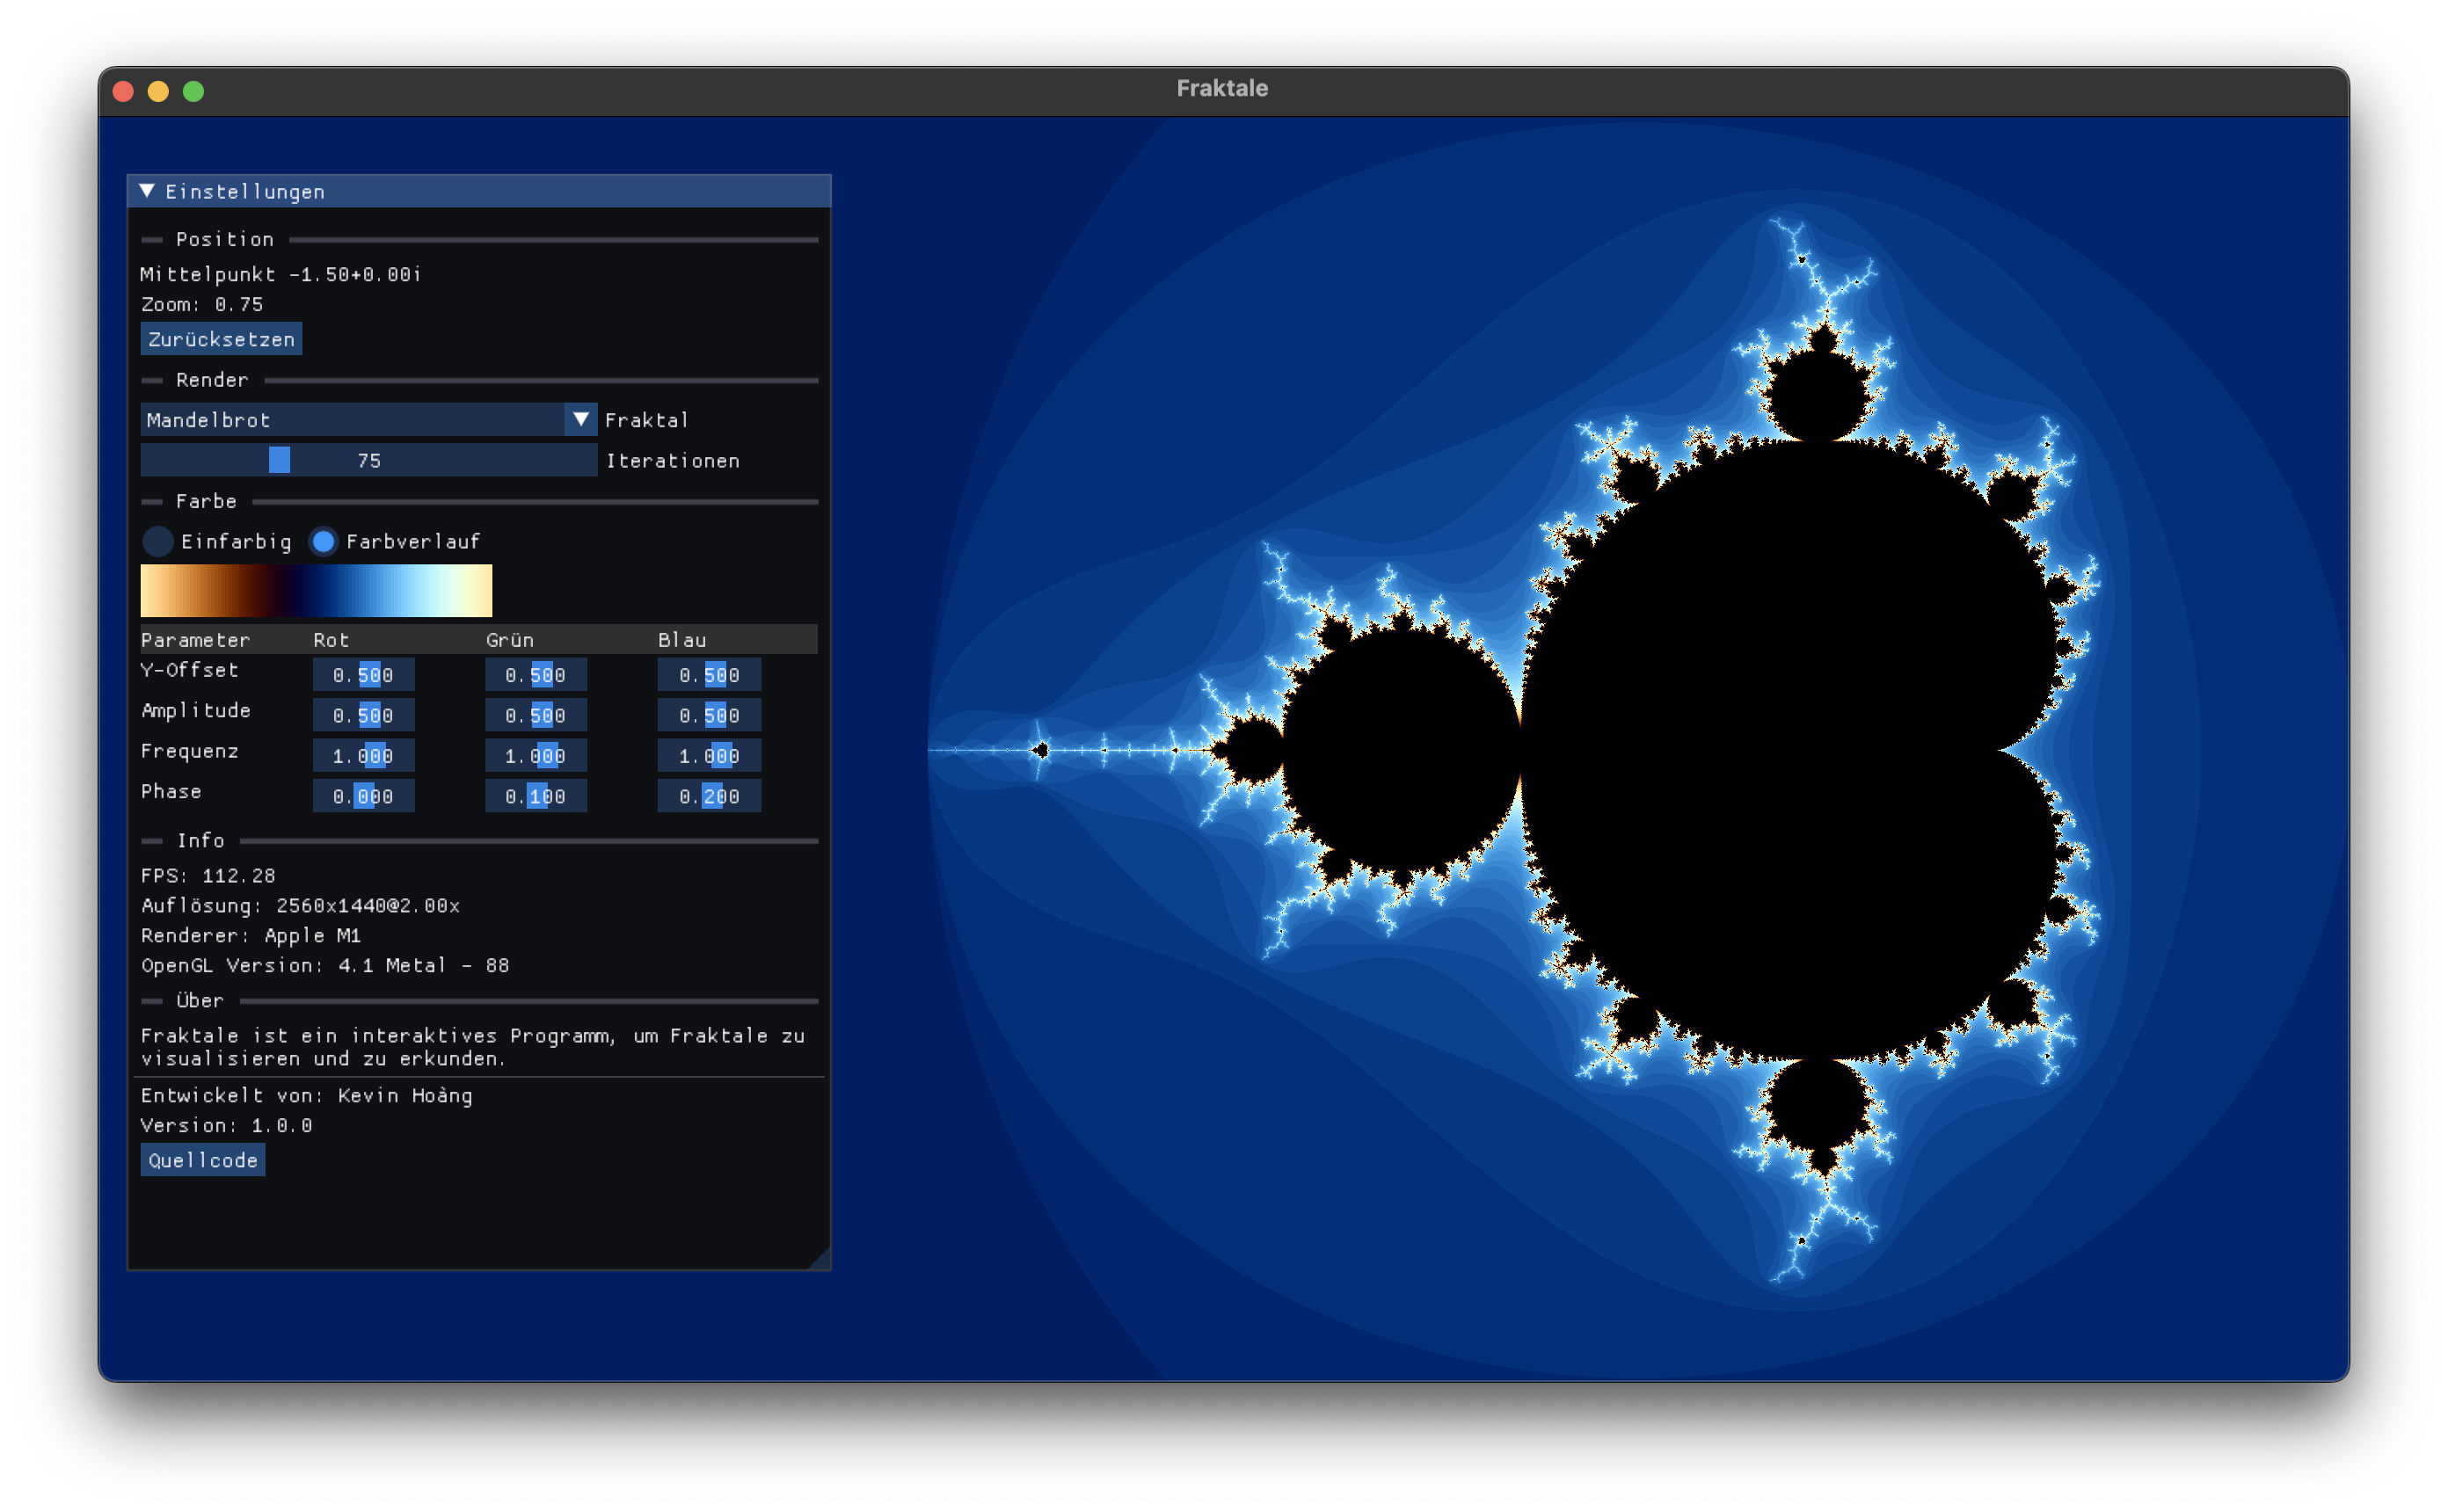
\includegraphics[width=0.8\textwidth]{img/Programm.png}
    \caption{Das Programm \textit{Fraktale}}
\end{figure}

\section{Programmaufbau}
Das Programm wurde in der Programmiersprache \textit{C++} geschrieben und nutzt
die Programmierschnittstelle \textit{OpenGL} um eine effiziente und
leistungsstarke Umsetzung der Algorithmen zu ermöglichen. Die Algorithmen
wurden in Form von \textit{Shadern} implementiert, die auf der Grafikkarte
ausgeführt werden. Diese werden in der Programmiersprache \textit{GLSL}
geschrieben. \newline C++ und GLSL sind bezüglich Syntax sehr ähnlich, was das
Deklarieren von Variablen und Funktionen, sowie Berechnungen betrifft.\hfill
\break \newline \noindent Zusätzlich wurden Bibliotheken verwendet, deren
genauere Beschreibung und Funktion sich im Anhang befindet. \hfill \break
\newline \noindent Das Programm besteht aus folgenden Dateien:
\begin{itemize}
    \item \texttt{main.cpp} - Die Hauptdatei, in der das Programm initialisiert wird.
    \item \texttt{window.h} - In dieser Datei befinden sich Funktionen, die das Fenster erstellen und verwalten.
    \item \texttt{dearimgui.h} - In dieser Datei befinden sich Funktionen, um die Benutzeroberfläche zu erstellen und zu verwalten.
    \item \texttt{callbacks.h} - In dieser Datei befinden sich Funktionen, um die Fraktale mit der Maus zu verschieben und zu zoomen.
    \item \texttt{shader.h / shader.cpp} - Eine Hilfsdatei, die das Laden und Kompilieren von Shadern ermöglicht.
    \item \texttt{misc.h} - Eine Hilfsdatei, die Funktionen enthält, die in anderen Dateien verwendet werden.
    \item \texttt{VertexShader.vert} - Der Vertex Shader, welcher für die Positionierung der \textit{Vertices} zuständig ist.
    \item \texttt{FragmentShader.frag} - Der Fragment Shader, wo die eigentliche Berechnung des Fraktals stattfindet.
\end{itemize}

\section{Implementierung der Algorithmen}

\blindtext

% \section{Limitationen} %